% \begin{figure}[htbp]
%   \centering
 
%   \begin{subfigure}{1.0\textwidth}
%     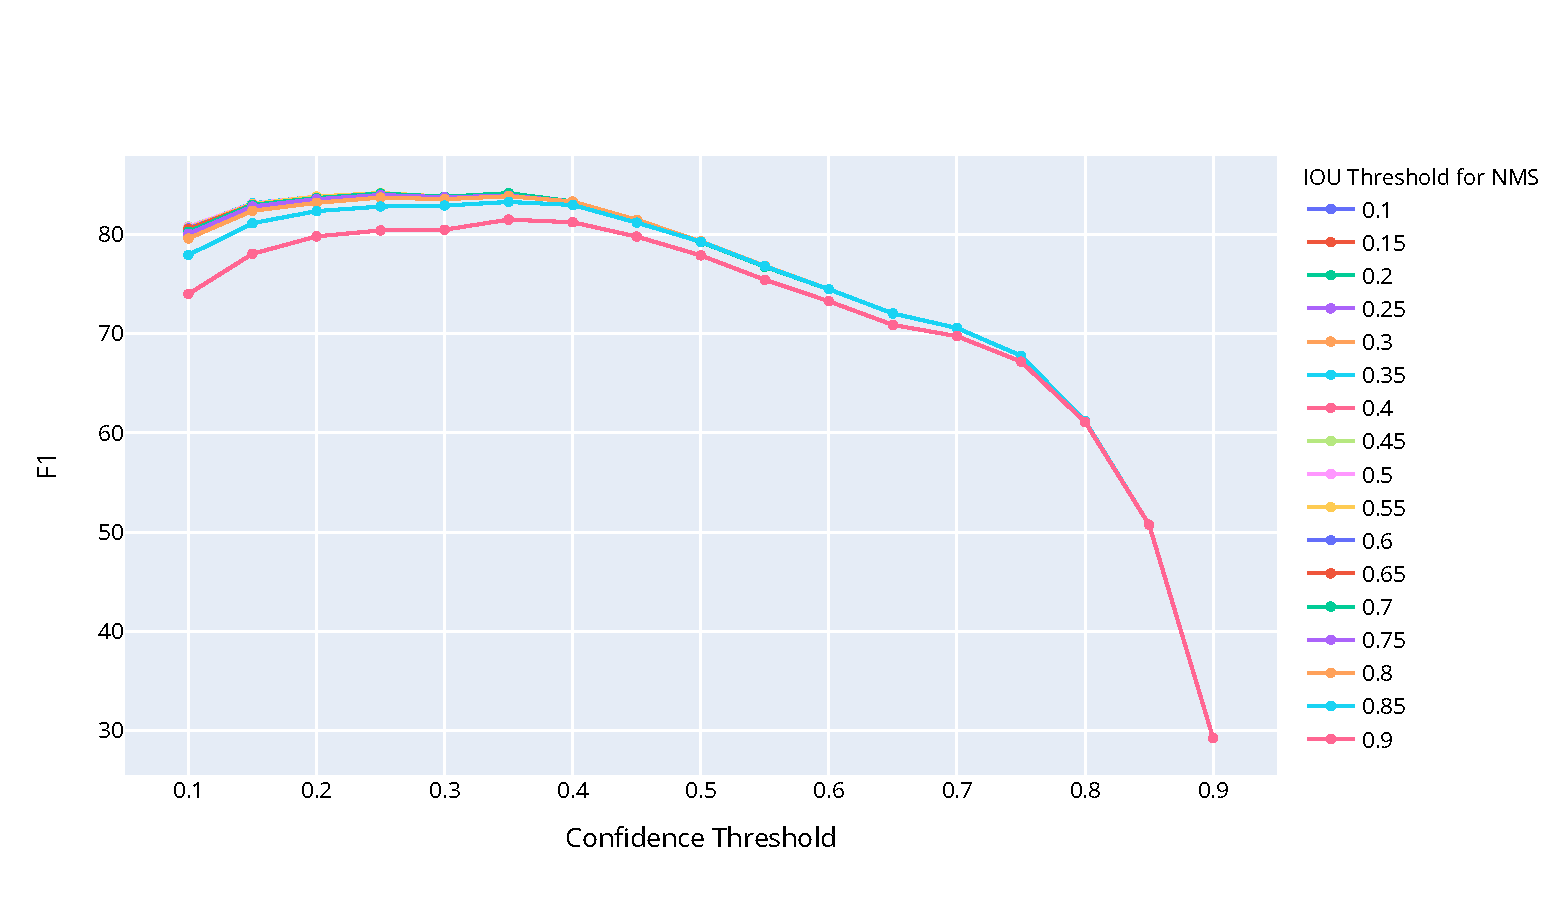
\includegraphics[width=\linewidth]{img/F1_vs_conf_plot.pdf}
%     \caption{F1 vs confidence threshold over different IOU threshold plot}
%     \label{fig:F1_vs_conf_plot}
%   \end{subfigure}
 
%     \bigskip
 
%   \begin{subfigure}{1.0\linewidth}
%     \centering
%     \resizebox{0.5\linewidth}{!}{
%     \begin{tabular}{rrr}
%     \toprule
%      Confidence Threshold &  IOU threshold for NMS &    F1 \\
%     \midrule
%                      0.25 &                   0.35 & 84.20 \\
%                      0.25 &                   0.40 & 84.20 \\
%                      0.25 &                   0.45 & 84.20 \\
%                      0.25 &                   0.50 & 84.20 \\
%                      0.25 &                   0.55 & 84.20 \\
%     \bottomrule
%     \end{tabular}
%     }
%     \caption{Highest F1 score on different confidence and IOU threshold}
%     \label{fig:F1_vs_conf_table}
%   \end{subfigure}
  

%   \caption{}
%   \label{fig:F1_vs_conf} % label should be placed below caption
% \end{figure}


%https://tex.stackexchange.com/questions/278574/common-caption-below-vertically-centered-figure-and-table

\begin{figure}
\centering

\begin{tabular}{@{}c@{}}
\resizebox{0.5\linewidth}{!}{
  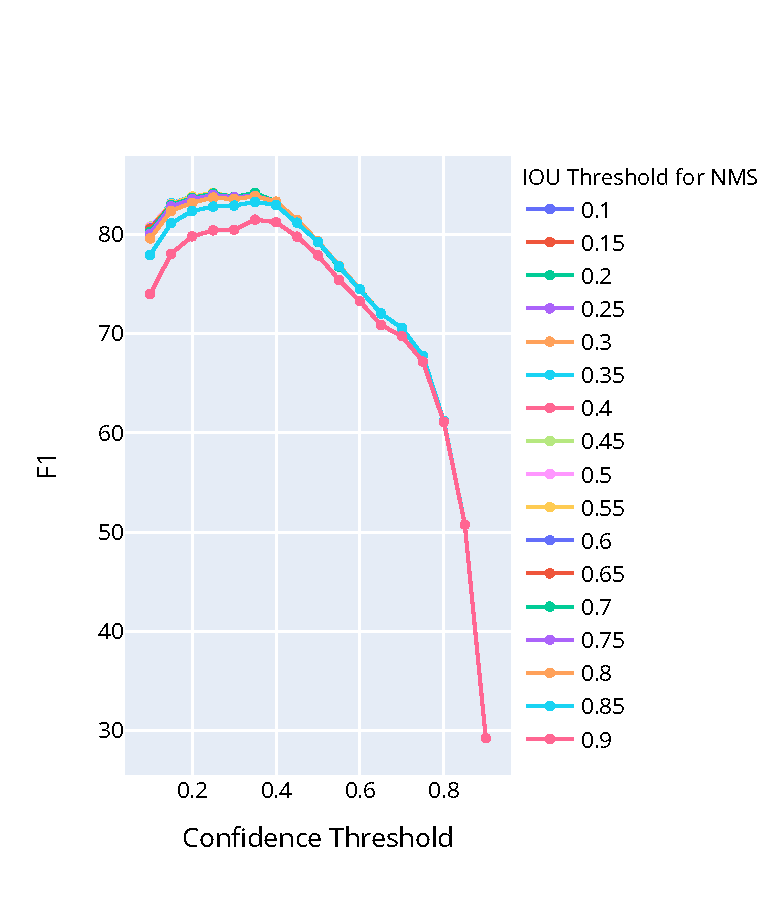
\includegraphics{img/optimizing_detector.pdf}}
\end{tabular}\qquad
\resizebox{0.4\linewidth}{!}{
\begin{tabular}{rrr}
\toprule
 Confidence Threshold &  IOU threshold for NMS &    F1 \\
\midrule
                 0.25 &                   0.35 & 84.20 \\
                 0.25 &                   0.40 & 84.20 \\
                 0.25 &                   0.45 & 84.20 \\
                 0.25 &                   0.50 & 84.20 \\
                 0.25 &                   0.55 & 84.20 \\
\bottomrule
\end{tabular}
}

\caption{A caption for a figure in a figure and a table side by side}\label{fig:optimizing_detector}
\end{figure}